\def\duedate{12/08/22}
\def\HWnum{4}
% Document setup
\documentclass[12pt]{article}
\usepackage[margin=1in]{geometry}
\usepackage{fancyhdr}
\usepackage{lastpage}

\pagestyle{fancy}
\lhead{Richard Whitehill}
\chead{PHYS 714 -- HW \HWnum}
\rhead{\duedate}
\cfoot{\thepage \hspace{1pt} of \pageref{LastPage}}

% Encoding
\usepackage[utf8]{inputenc}
\usepackage[T1]{fontenc}

% Math/Physics Packages
\usepackage{amsmath}
\usepackage{amssymb}
\usepackage{dsfont}
\usepackage{mathtools}
\usepackage[arrowdel]{physics}
\usepackage{siunitx}

\AtBeginDocument{\RenewCommandCopy\qty\SI}

% Reference Style
\usepackage{hyperref}
\hypersetup{
    colorlinks=true,
    linkcolor=blue,
    filecolor=magenta,
    urlcolor=cyan,
    citecolor=green
}

\newcommand{\eref}[1]{Eq.~(\ref{eq:#1})}
\newcommand{\erefs}[2]{Eqs.~(\ref{eq:#1})--(\ref{eq:#2})}

\newcommand{\fref}[1]{Fig.~\ref{fig:#1}}
\newcommand{\frefs}[2]{Figs.~\ref{fig:#1}--\ref{fig:#2}}

\newcommand{\tref}[1]{Table~\ref{tab:#1}}
\newcommand{\trefs}[2]{Tables~\ref{tab:#1}-\ref{tab:#2}}

% Figures and Tables 
\usepackage{graphicx}
\usepackage{float}

\newcommand{\bef}{\begin{figure}[h!]\begin{center}}
\newcommand{\eef}{\end{center}\end{figure}}

\newcommand{\bet}{\begin{table}[h!]\begin{center}}
\newcommand{\eet}{\end{center}\end{table}}

% tikz
\usepackage{tikz}
\usetikzlibrary{calc}
\usetikzlibrary{decorations.pathmorphing}
\usetikzlibrary{decorations.markings}
\usetikzlibrary{arrows.meta}
\usetikzlibrary{positioning}

% tcolorbox
\usepackage[most]{tcolorbox}
\usepackage{xcolor}
\usepackage{xifthen}
\usepackage{parskip}

\newcommand*{\eqbox}{\tcboxmath[
    enhanced,
    colback=black!10!white,
    colframe=black,
    sharp corners,
    size=fbox,
    boxsep=8pt,
    boxrule=1pt
]}

% Miscellaneous Definitions/Settings
\newcommand{\prob}[2]{\textbf{#1)} #2}

\setlength{\parskip}{\baselineskip}
\setlength{\parindent}{0pt}

\def\complexs{\mathbb{C}}
\def\reals{\mathbb{R}}
\def\naturals{\mathbb{N}}
\def\integers{\mathbb{Z}}
\def\rationals{\mathbb{Q}}
\def\id{\mathds{1}}



\begin{document}
    
\prob{1}{
Given matrix
\begin{eqnarray}
    A = \begin{pmatrix}
        0 & -1 & 0 & 1 \\
        0 & 1 & 0 & 1 \\
        1 & 0 & 1 & 1 \\
        1 & 0 & 0 & -1
    \end{pmatrix}
.\end{eqnarray}
Without the calculation of eigenvalues, please answer the following questions.
}

a) What is the sum of the eigenvalues of $A$?

The sum of the eigenvalues of a matrix is equal to the trace of $A$:
\begin{eqnarray}
    \lambda_{1} + \lambda_{2} + \lambda_{3} + \lambda_{4} = \Tr(A) = 0 + 1 + 1 + -1 = 1
.\end{eqnarray}

b) What is the product of the eigenvalues of $A$?

The product of eigenvalues is just the determinant of $A$, which was determined using wolfram:
\begin{eqnarray}
    \lambda_1\lambda_2\lambda_3\lambda_4 = \det(A) = -2
.\end{eqnarray}


c) What's your observation of the eigenvalues of $A A^{\rm T}$?

The eigenvalues of $A A^{\rm T}$ multiply to be the square of the product of eigenvalues of $A$: $\det(A A^{\rm T}) = \det^2(A)$

\prob{2}{
For $n \times n$ real symmetric matrices $A$ and $B$, prove $AB$ and $BA$ always have the same eigenvalues.
}

Let $\lambda$ be an eigenvalue of the matrix $AB$.
Then, by definition, $\lambda$ solves the equation $\det(AB - \lambda \id) = 0$.
Note that $\det(AB - \lambda \id) = \det[(AB - \lambda \id)^{\rm T}] = \det((AB)^{\rm T} - \lambda \id) = \det(BA - \lambda\id) = 0$.
That is, $AB$ and $BA$ have the same characteristic equation, implying that their eigenvalues are the same.

\prob{3}{
For $n \times n$ matrices $A$ and $B$ prove $AB$ and $BA$ always have the same eigenvalues if $B$ is invertible.
}

Note that similar matrices have the same eigenvalues, and since $B$ is invertible $AB$ is similar to $B(AB)B^{-1} = BA$, which implies that $AB$ and $BA$ have the same eigenvalues if $B$ is invertible.

\prob{4}{
Starting with a random matrix $A \in \reals^{100 \times 100}$, perform $QR$ iteration 200 times.
Plot the sparsity pattern for initial matrix $A$ and final output matrix.
}

The code is shown below with the result.
Note that we initialized our random matrix with integers between $-5$ and $5$.
For the sparsity pattern, the dots represent nonzero entries while white space represents an effectively zero entry (i.e. $A_{ij} < 10^{-10}$).
It is clear that the $QR$ iteration transforms $A$ into an upper triangular matrix.

\inputpython{prob4.py}

\begin{center}
    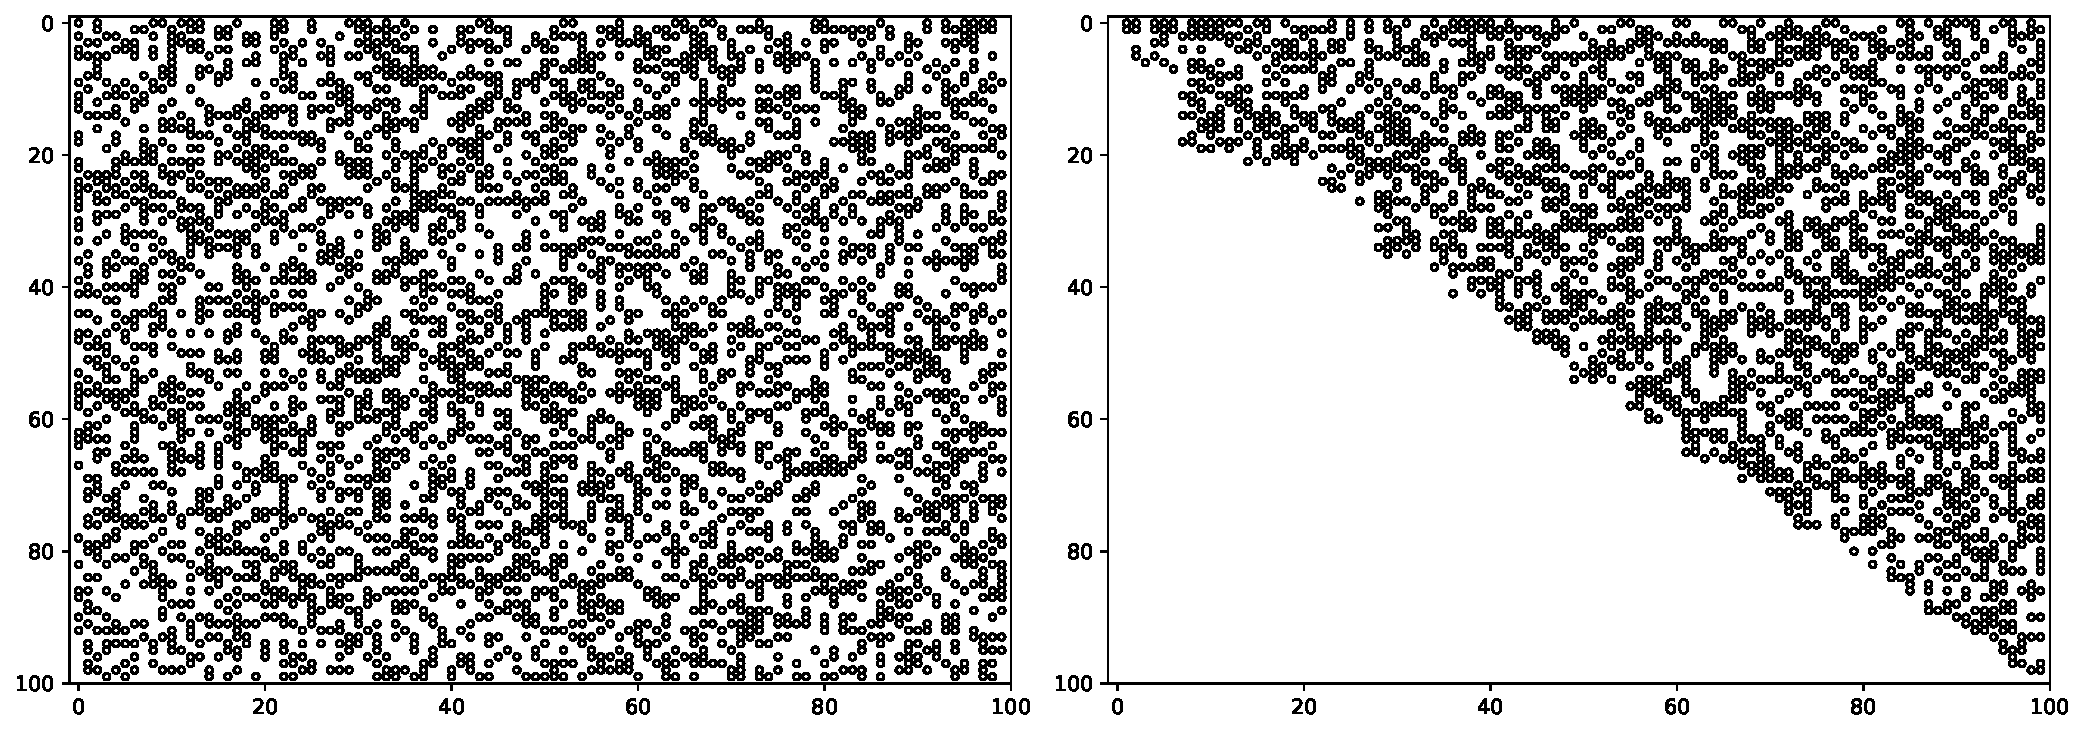
\includegraphics[width=0.7\textwidth]{prob4.pdf} 
\end{center}

\prob{5}{
Consider $A \in \reals^{10 \times 10}$ of the form
\begin{eqnarray}
    A = \begin{pmatrix}
        2 & -1 & & & \\
        -1 & 2 & -1 & & \\
           & \ddots & \ddots & \ddots & \\
           & & \ddots & \ddots & -1 \\
           & & & -1 & 2
    \end{pmatrix}
.\end{eqnarray}
}

a) Implement the power method to compute an approximation to the eigenvalue of largest absolute value and its corresponding eigenvector, starting with a random initial vector and stop the iteration with relative error $10^{-6}$.

The code an results for this part are shown below:

\inputpython{prob5a.py}
\begin{center}
    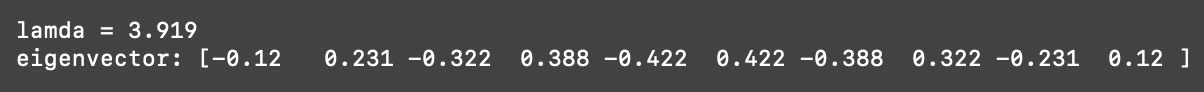
\includegraphics[width=0.8\textwidth]{prob5a.png}
\end{center}

b) Implement the $QR$ algorithm (without shifts) to convert $A$ to diagonal form and find out all the eigenvalues.

The code implementing the ``basic'' $QR$ algorithm without shifts for calculation of the eigenvalues is shown below along with a screenshot of the resultant eigenvalues.

\inputpython{prob5b.py}
\begin{center}
    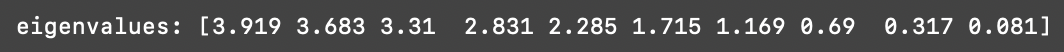
\includegraphics[width=0.8\textwidth]{prob5b.png}
\end{center}

c) Take the 5th eigenvalue computed in your $QR$ algorithm and, using it as a fixed shift in inverse iteration, compute the corresponding eigenvector.

The code implementing the inverse power method to calculate the eigenvector corresponding to the the 5th eigenvalue calculated in part (b) is shown below along with a screenshot of the output.

\inputpython{prob5c.py}
\begin{center}
    
\includegraphics[width=0.8\textwidth]{prob5c.png}
\end{center}


\end{document}
